\documentclass[12pt,a4paper]{article}

\usepackage{color}
\usepackage{amsxtra}  
\usepackage{amsthm}
\usepackage{amssymb}
\usepackage{amsfonts}
\usepackage{graphicx}  
\usepackage{rotating}


\begin{document}

\title{Report: Characteristics of pinned polymer loop in external field}
\author{Wenwen Huang}
\date{\today}

\maketitle

\section{Motivation}
\label{sec:motivation}

During meiosis I in Fission Yeast (S. pombe), a dramatic chromosome movement
named nuclear oscillation is observed. Spindle Pole Body (SPB), which is a
centrosome like organelle embedded in the nucleus membrane and bonded to the
microtubes out of nucleus, drives the nucleus moves forward and backward in the
cylinder shaped cell. Chromosomes in the nucleus, which are of course moving
together, are aligned and recombined during this $2-3$ hours period. 

Chromosomes with both ends bound to SPB can be modelled by polymer loops. Consider
the time window of one-direction moving of nucleus, hydrodynamical interaction between
cytoplasm and chromosomes acts as an external force field on every spot of the
loop. Transform to a co-moving frame (sitting on the SPB), the movement of
chromosomes in one direction maps to the scenario of pinned polymer loops in
external force field. Since the moving speed of nucleus in one direction is
nearly steady (observed in experiments), the corresponding force field can be
considered as constant.

There are three pairs of homologous in fission yeast nucleus. Morphology state
of these chromosomes are believed to be important to biological functionalities
such as recombination. We therefore want to study the characteristics of these
chromosomes during nuclear oscillation. More specifically, I assume the shape
of the nucleus is determined by the morphology of chromosomes (to be justified).
With this assumption, it is possible to compare the prediction to experiments. 
Using both theoretical and simulation tools, several characteristic parameters
of polymer loops in external force field can be calculated quantitatively.  

\section{Model}
\label{sec:model}
Pinned polymer loops in external force field is used to describe chromosomes.
As shown in Figure \ref{fig:sketch}. The 
\begin{figure}[htpb]
	\centering
	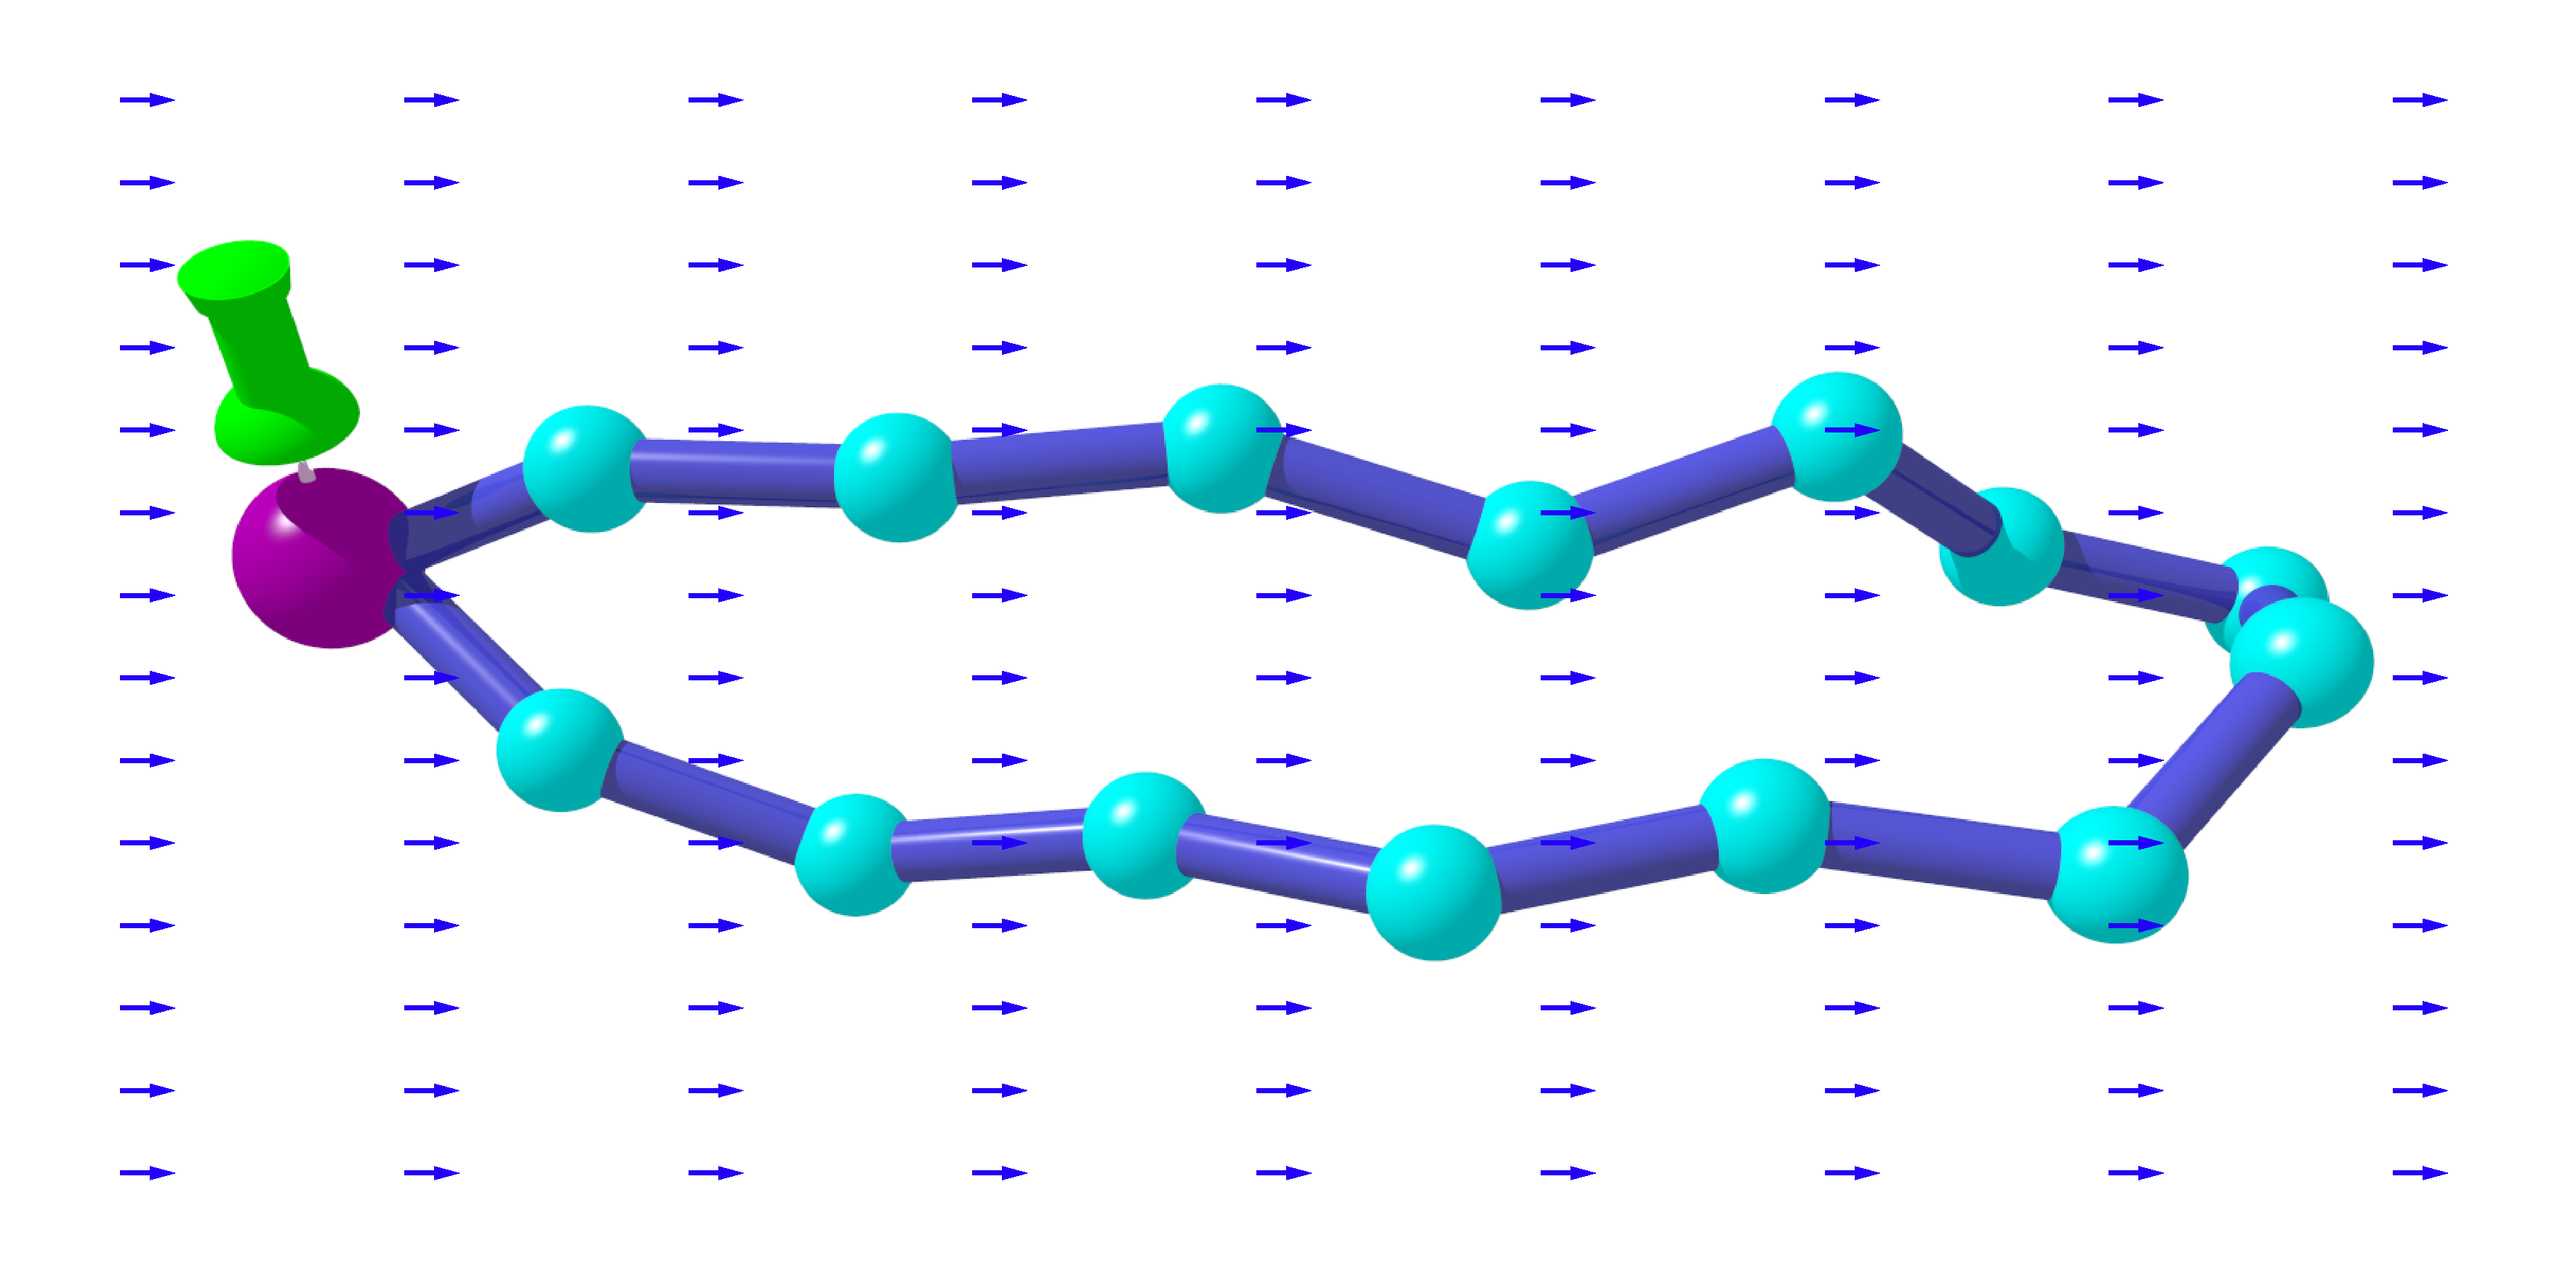
\includegraphics[width=0.8\linewidth]{sketch}
	\caption{Sketch of polymer loop representing chromosomes. Magenta bead
		represents the SPB.}
	\label{fig:sketch}
\end{figure}

\section{Simulation}
\label{sec:simulation}

\section{Results}
\label{sec:results}

\section{Discussion}
\label{sec:discussion}




\end{document}
